\section{Enumeration Method}

\textbf{Probleme mit Iterator}

\begin{itemize}
	\item Iterator und Collection sind stark gekoppelt
	\item Aufwendiges Lifecycle Management notwendig; Iterator muss Collection überwachen
\end{itemize}

\textbf{Alternative zu Iterator}

Kapsle Iterationslogik über eine Collection in eine Enumeration Method der Collection, die ein Command Object mit der Verarbeitungslogik entgegennimmt.

Auch als Internal Iterator bekannt, jedoch nur selten berücksichtigt.

\begin{figure}[H]
	\centering
	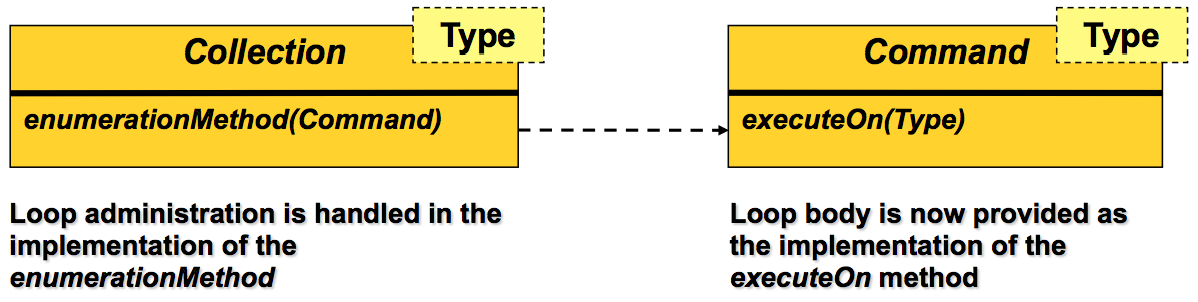
\includegraphics[width=0.9\textwidth]{content/advancedPatterns/enumerationmethod.png}
	\caption{Enumeration Method}
\end{figure}

\textbf{Konsequenzen}

\begin{itemize}
	\item Client ist nicht für die Verwaltung eines Iterators zuständig
	\item Synchronisation kann für die gesamte Traversierung gewährleistet werden, statt nur pro Zugriff
	\item Führt zum Teil zu unnötig viel Code und Verschmutzung des Namespaces da viele Command Objekte benötigt werden
	\item Kann u.U. zur Verwirrung führen; ``zu abstrakt''
\end{itemize}


\section{State Patterns}

\textbf{Objects for States}

Siehe GoF State Pattern

\textbf{Methods for States}

Stelle jeden Zustand als Tabelle von Methoden oder Funktionen dar, die über diese Tabelle aufgerufen werden.

\textbf{Konsequenzen}

\begin{itemize}
	\item Das Verhalten eines Objekts kann vollständig innerhalb der Klasse definiert werden (als private Methods); keine ``Verzettelung'' wie bei Objects for States
	\item Methodenaufrufe werden zusätzlich umgeleitet; Performanceeinbussen
	\item Teilen von Verhalten zwischen unterschiedlichen Zuständen ist sehr einfach
	\item Vertehen der Klasse wird schwieriger, da das genaue Verhalten in einem Zustand durch den Leser aufgeschlüsselt werden muss
	\item Nur geeignet in Sprachen, die das referenzieren und auflösen von Methoden einfach unterstützen. z.B. C++, Scala, Ruby im Gegensatz zu Java
\end{itemize}

\textbf{Collections for States}

Gruppiere Objekte im selben Zustand in Collections sodass der State durch dazugehörigkeit zu einer Collection repräsentiert wird. So können z.B. in einem Editor, der mehrere Dateien bearbeitet, alle veränderten Dateien in einer Collection ``changed'' abgelegt werden und alle unveränderten in der Collection ``saved''. Um nun alle Dateien zu speichern kann über alle ``changed'' Dateien iteriert werden, welche anschliessend nach ``saved'' verschoben werden.

\textbf{Konsequenzen}

\begin{itemize}
	\item Aktionen über alle Aktionen eines bestimmten States sind effizient durchführbar
	\item Bei Systemen mit beschränkten Ressourcen kann der Memory Footprint pro Objekt u.U. verringert werden, da der State implizit über die Collectionzugehörigkeit bestummen wird
	\item Es können unterschiedliche Zustandsmodelle auf Objekte angewendet werden, ohne diese zu erweitern
	\item Der Manager bekommt mehr Verantwortung als beim Objects for States Pattern
	\item Das halten von Zustandsabhängigen Daten für die Objekte ist schwieriger
\end{itemize}

\section{Value Patterns}

\textbf{Objektmerkmale}

Objekte können nach drei Aspekten charakterisiert werden:

\begin{itemize}
	\item Identität
	\item Zustandslos / Zustandsbehaftet
	\item Verhalten
\end{itemize}

Eine mögliche Kategorisierung von Objekten ist:

\begin{itemize}
	\item Entity - Drücken Systeminformationen aus und werden oft persistiert; Identität ist wichtig
	\item Service - Kapseln Systemaktivitäten; Werden anhand ihres Verhaltens auseinandergehalten
	\item \textbf{Value} - Werden durch ihren Inhalt charakterisiert; haben keine dauerhafte Identität; ``existieren ausserhalb von Raum und Zeit''
	\item Task - Stellen ebenfalls Systemaktivitäten dar, verfügen jedoch über einen Zustand und eine Identität
\end{itemize}

\subsection{Immutable Value}

Wie können Objekte ohne Probleme wegen Seiteneffekten / Nebenläufigkeit etc. geteilt werden?

Definiere Typen, deren Instanzen nur über nicht mutable Attribute verfügen. Der interne Zustand der Objekte wird während der Konstruktion gesetzt und ändert nicht mehr. Änderungen am Zustand müssen über das Erzeugen von neuen Objekten geschehen.

Verwende das ``final'' Schlüsselwort für Attribute in Java. Vorsicht: sind Attribute Objekttypen, so müssen diese ebenfalls Immutable sein!

\subsection{Whole Value}

Wie können Mengen oder Grössen dargestellt werden, ohne deren Bedeutung zu verlieren? Primitive Datentypen verfügen nicht über Einheiten und bieten nur rudimentäre Typprüfung zur Compilezeit.

Erstelle eine Klasse um die Menge auszudrücken (z.B. Date) und Kapsle so ein oder mehrere primitive Werte.

Wichtig in Java: boolean equals(Object o), int hashCode() und Serializable falls angebracht. toString() kann ebenfalls nützlich sein.

\subsection{Enumeration Values}

Wie kann eine geschlossene Menge von konstanten Werten typsicher abgebildet werden (z.B. Monate)?

Behandle alle Werte als konstante Whole Values und verhindere public Construction (Enum in vielen Sprachen).

\subsection{Class Factory Method}

Wie kann die Konstruktion von Value Objects vereinfacht und auf ``new'' Ausdrücke verzichtet werden?

Benutze eine statische Methode für die Werterzeugung. Dies ist eine Variation von Factory Method, einfach dass die Factory Methode nur Instanzen der eigenen Klasse erzeugt.

\begin{lstlisting}[language=Java, caption={Class Factory Method}]
Date clumsy = new Date(new Year(2013), new Month(12), 30); // umständlich, keine Möglichkeit um Values wiederzuverwenden
Date dangerous = new Date(2013, 4, 5); // keine Typsicherheit / Verwechslungsgefahr

Date nice = new Date(Year.valueOf(2012), Month.valueOf(2), 30);
\end{lstlisting}

\subsection{Mutable Companion}

Wie kann die Konstruktion von komplexen Immutable Objects vereinfacht werden? z.B. das Datum 15 Arbeitstage nach Übermorgen

Benutze eine Companion Class für die Erstellung der Immutable Objects, wie z.B. StringBuffer und StringBuilder für Java Strings.


\section{Reflection Patterns}

\subsection{Type Object}

Wie können Objekte dynamisch kategorisiert werden obwohl kein genügend flexibles Typsystem zur Verfügung steht?

Markiere Objekte mit anderen Objekten statt einer Klasse, sodass neue Kategorien zur Laufzeit hinzugefügt werden können.

Objekte delegieren Serviceanfragen an ihren ``Typ''. Dieser kann durch den Client beliebig ausgewechselt werden, wobei die Objektidentität immer gewahrt ist.

\begin{figure}[H]
	\centering
	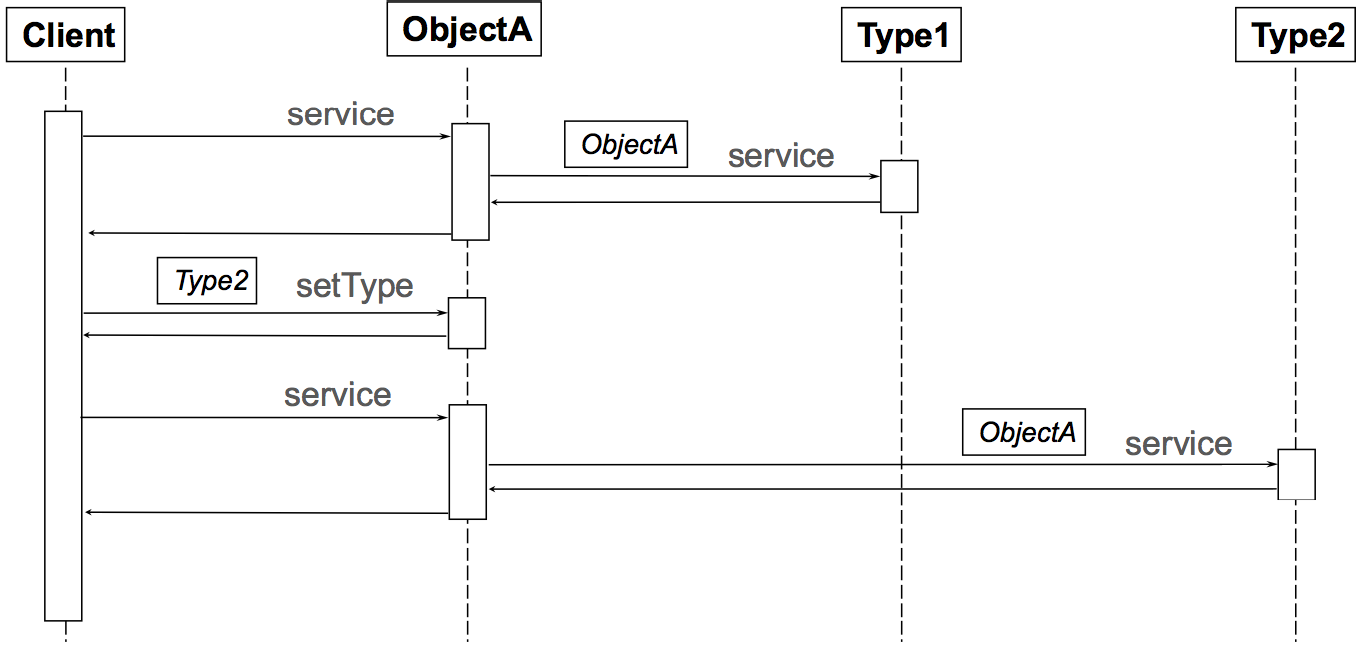
\includegraphics[width=0.9\textwidth]{content/advancedPatterns/typeobject.png}
	\caption{Type Object funktionsweise}
\end{figure}

\begin{itemize}
	\item Neue Kategorien sind einfach hinzufügbar, auch zur Laufzeit
	\item Verhindert unzählige triviale Unterklassen
	\item Mehrere Meta Levels möglich (Typobjekte für Typobjekte)
	\item Verwirrung wegen Separation
	\item Effizienzeinbussen wegen Indirektion
\end{itemize}

\subsection{Property List}

Wie können Attribute flexible zur Laufzeit zu Objekten hinzugefügt/entfernt werden? z.B. in einem Shop Items mit unterschiedlichen Attributen je nach Kategorie.

Erweitere die Objekte um eine Property List in Form einer Map Attributname -> Wert.

\begin{itemize}
	\item Objekt kann erweitert werden während Identität erhalten bleibt
	\item Falls alle Attribute in der Property List enthalten sind, kann die Persistierung einfach und ohne Sprachspezifische Reflexion umgesetzt werden
	\item Methoden können mit flexiblen Parametern aufgerufen werden
	\item Unterschiedliche Arten um auf reguläre und flexible Attribute zuzugreifen
	\item Type Safety muss durch den Programmierer gewährleistet werden
	\item Attributnamen werden nicht vom Compiler überprüft
	\item Bedeutung von Attributen ist nicht durch die Klasse definiert
	\item Hoher Overhead
\end{itemize}

\subsection{Anything}

Wie können Methodenparameter definiert werden, die die Anforderungen von zukünftigen Subklassen erfüllen? Wie gestaltet man einen flexiblen, strukturierten Konfigurationsmechanismus der einfach erweiterbar ist? Wie kann die Datenstruktur, die zwischen Subsysteme ausgetauscht wird, angepasst werden, ohne dass alle Subsysteme neu kompiliert werden müssen?

Erstelle eine selbstbeschreibende, strukturierte Datenstruktur die über ein einfach lesbares externes Textformat verfügt (z.B. als XML oder JSON Dokument).

\begin{figure}[H]
	\centering
	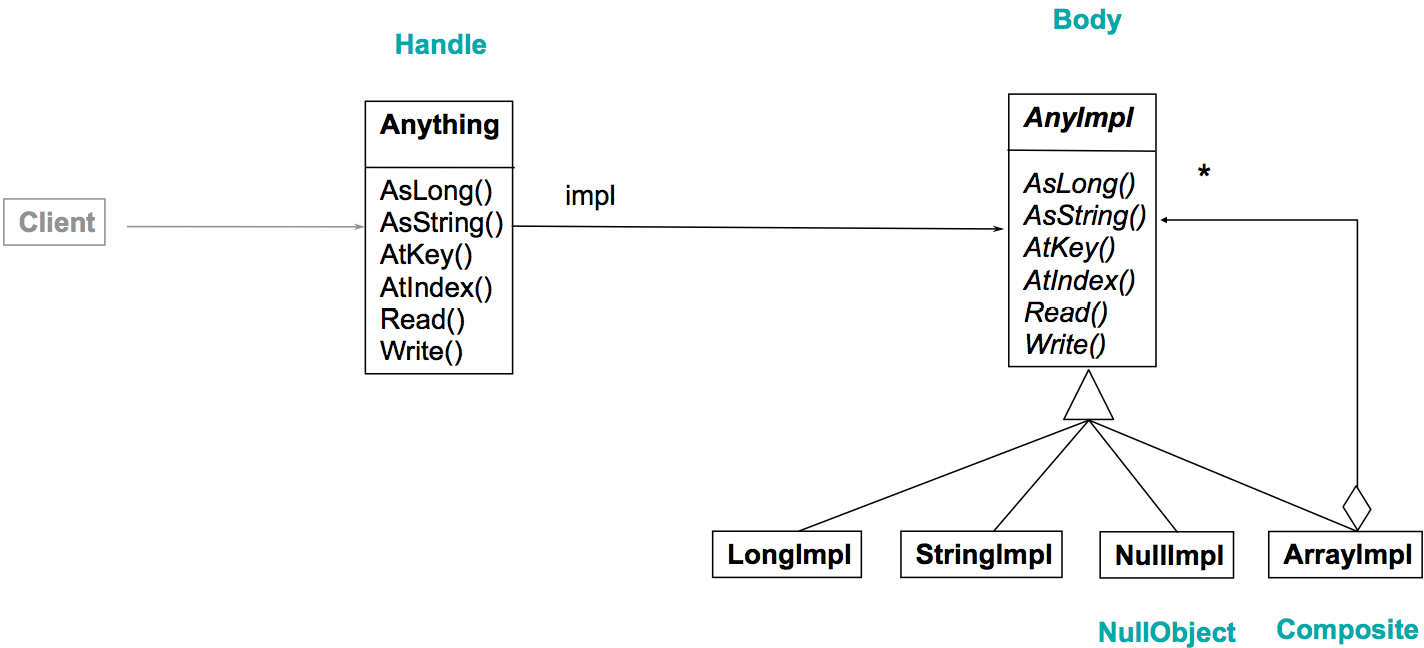
\includegraphics[width=0.9\textwidth]{content/advancedPatterns/anything.png}
	\caption{Anything}
\end{figure}

\begin{itemize}
	\item Einfach benutzbar
	\item Lesbares externes Format -> gut für Konfigurationen
	\item Universell und flexibel über Klassengrenzen einsetzbar
	\item Erlaubt einfache aber brauchbare Interfaces ohne Methodenüberladung
	\item Verminderte Typsicherheit
	\item Zweck von Parametern nicht immer erkennbar
	\item Performanceoverhead
	\item Nicht wirklich Objekte, nur Daten (keine spezifischen Methoden)
\end{itemize}

\subsection{Extension Interface}

\begin{itemize}
	\item Alter Client Code soll bei Erweiterungen von Komponenten nicht betroffen sein, idealerweise auch nicht neu kompiliert werden müssen!
	\item Hinzufügen von neuer, spezifischer Funktionalität zur Klassenhierarchie kann zum ``Fragile Base Class'' Problem führen (Hinzufügen von Methoden in der Basisklasse führt in Subklassen zu Fehlfunktionen)
	\item Interfaces können nur schwer für noch unbekannte Szenarien entworfen werden
	\item Neue Funktionalitäten sollen nicht zu Overhead bei alten Clients führen, die diese gar nicht benötigen
\end{itemize}

Wie können die Komponenten trotzdem für zukünftige Erweiterungen offen entworfen werden?

Clients sollen auf Komponenten via einzelne Interfaces Zugreifen statt das die Komponente alle Funktionalitäten über ein Interface zur Verfügung stellt. Jedes Interface steht für eine Rolle, die die Komponente einnehmen kann. Clients haben somit nur Abhängigkeiten zu den Rollen der Komponente, die sie auch benutzen.

Alle ExtensionInterfaces müssen zudem von einem RootInterface erben, über welches der Client auf weitere ExtensionInterfaces der Komponente zugreifen können.

\begin{figure}[H]
	\centering
	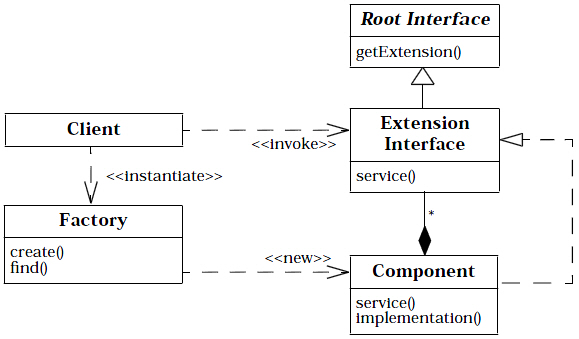
\includegraphics[width=0.6\textwidth]{content/advancedPatterns/extensioninterface.jpg}
	\caption{Extension Interface}
\end{figure}

\begin{description}
	\item[Component] Implementiert und aggregiert Service Funktionalitäten von mindestens einem Extension Interface; kann verschiedene Rollen einnehmen
	\item[Root Interface] Definiert die Funktionalität, die jede Komponente mindestens zur Verfügung stellen muss; typischerweise eine getExtension(InterfaceId) Methode
	\item[Extension Interface] Definiert rollenspezifische Funktionalitäten, die eine Komponente implementieren kann
	\item[Client] Benutzt Factories um neue Components zu erhalten und benutzt diese über die Extension Interfaces
	\item[Component Factory] Erzeugt Komponenten oder bietet Zugriff auf bereits existierende Komponenten
\end{description}

\begin{figure}[H]
	\centering
	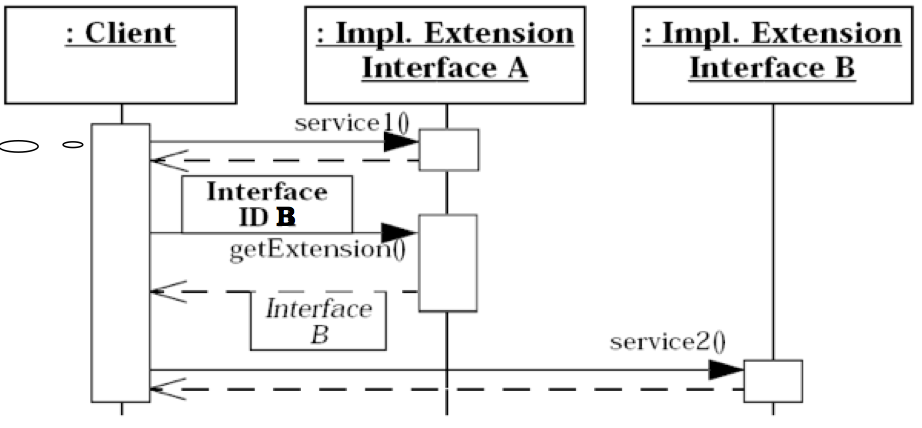
\includegraphics[width=0.6\textwidth]{content/advancedPatterns/extensioninterfaceusage.png}
	\caption{Zugriff auf Extension Interface}
\end{figure}

\textbf{Konsequenzen}

\begin{itemize}
	\item Erweiterbarkeit ohne aufgeblasene Interfaces
	\item Polymorphismus ohne dass das erben von einem gemeinsamen Interface notwendig ist
	\item Koppelung zwischen Clients und Komponenten wird verringert, da die Clients nur von den Extension Interfaces abhängig sind, die sie auch benutzen
	\item Komponente können Interfaces von anderen Komponenten aggregieren und diese als eigene Rollen anbieten und anschliessend delegieren
	\item Höhere Komplexität
	\item Zusätzliche Indirektion
\end{itemize}

\section{Encapsulated Context}

Wie können stetig wachsende Parameterlisten verhindert werden, die vor allem für das weiterreichen von oft bennötigten Services und Daten verwendet werden?

Sammle die entsprechenden Daten und Objekte in einem Context Objekt und reiche dieses von Funktion zu Funktion weiter. Als Context Objekt kann auch ein Anything oder eine PropertyList verwendet werden.

calc(receipt, logger, db, cmdOptions, ...);

Wird zu

calc(receipt, context);

Es können auch mehrere Context Objekte in einem System definiert werden, die jeweils 

\textbf{Konsequenzen}

\begin{itemize}
	\item Stabile Funktionssignaturen
	\item Globale Daten werden nicht mehr benötigt
	\item Instanzierung von Objekten im Context ist klar geregelt
	\item Gefahr, dass der Context zu einem Blob Objekt mit sehr geringer Kohärenz wird
	\item Gefahr von ``Hidden globals''
\end{itemize}


\section{Pooling}

